\documentclass{beamer}
\usepackage[utf8]{inputenc}
\usepackage{caption}
\usepackage{amsmath}
\usepackage{siunitx}
\usepackage{graphics,graphicx,amssymb,amsmath,pgf,comment,hyperref,gensymb}
\usepackage{fontspec}
\usepackage{anyfontsize}

\setmonofont{Roboto Mono Light}[
  Scale=MatchLowercase
]


\addtobeamertemplate{navigation symbols}{}{%
	\usebeamerfont{footline}%
	\usebeamercolor[fg]{footline}%
	\hspace{1em}%
	\insertframenumber/\inserttotalframenumber
	\setbeamercolor{footline}{fg=black}
}

\setbeamersize{text margin left=5mm,text margin right=5mm}
\subtitle{Momentum-Resolved Electron Energy-Loss Spectroscopy}
\title{Mapping of vibrations in graphene nanostructures}
\institute{AP3252 - Electron Microscopy - TU Delft}
\author{Jeroen Sangers}
\date{June 2022}



\begin{document}

\begin{frame}
	\titlepage
\end{frame}

% \begin{frame}
% 	\frametitle{Outline}
% 	\tableofcontents
% \end{frame}

\begin{frame}
	\frametitle{Content}
	\begin{itemize}
		\item Goal of the paper
  		\item Microscope modifications
    	\item Sample
     	\item Results
	\end{itemize}
\end{frame}

\begin{frame}
	\section{goal}
	\frametitle{Goal of the paper}
	\begin{minipage}{1\linewidth}
		\centering
		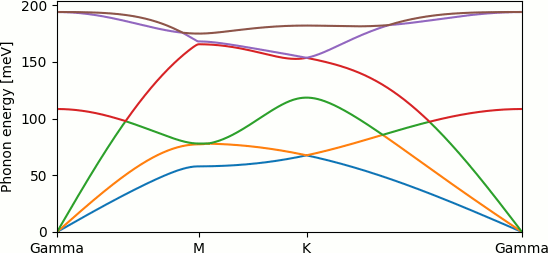
\includegraphics[width=.75\linewidth, keepaspectratio]{Figures/PhononDispersionGraphene.png}
	\end{minipage}%
	\hfill
	\begin{minipage}{1\linewidth}
		Shows:
		\begin{itemize}
			\item different bands $\rightarrow$ different modes
   			\item dispersion, set energy-momentum relation
      		\item crystallographic direction
		\end{itemize}
	\end{minipage}

\end{frame}

\begin{frame}
	\section{Technique}
	\subsection{The Microscope}
	\frametitle{Microscope set-up, Monochromator}
	\begin{minipage}{0.5\linewidth}
		\centering
		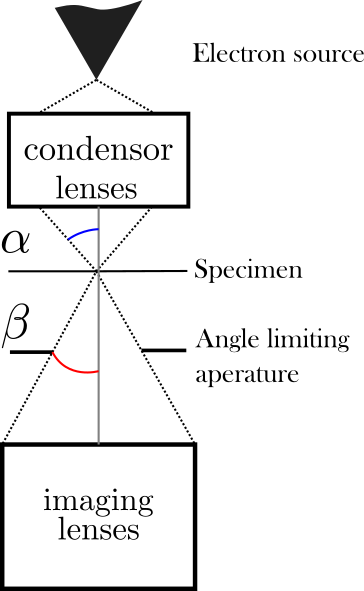
\includegraphics[width=0.7\linewidth, keepaspectratio]{Figures/tem.png}
	\end{minipage}%
	\begin{minipage}{0.5\linewidth}
		\centering
		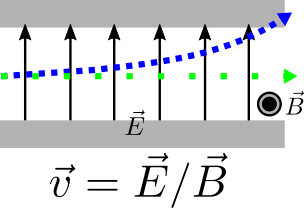
\includegraphics[width=0.7\linewidth, keepaspectratio]{Figures/monochromator.png}
	\end{minipage}
\end{frame}

\begin{frame}
	\frametitle{Microscope set-up, Spectrometer}
	\centering
	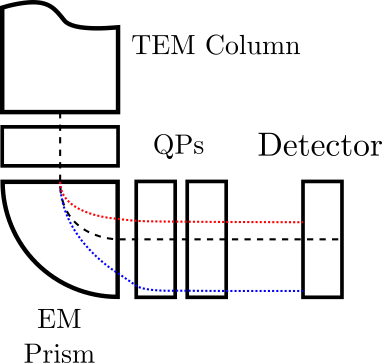
\includegraphics[width=0.6\linewidth, keepaspectratio]{Figures/prism.png}\\
	\vspace{0.5cm}
	Entrance aperture of $q=0.2 \si{\angstrom}^{-1}$ for beam size of $10nm$

\end{frame}

\begin{frame}
	\subsection{Momentum-resolved electron energy-loss spectroscopy}
	\frametitle{\textbf{Momentum-Resolved} EELS}
	\begin{minipage}{0.5\linewidth}
		\centering
		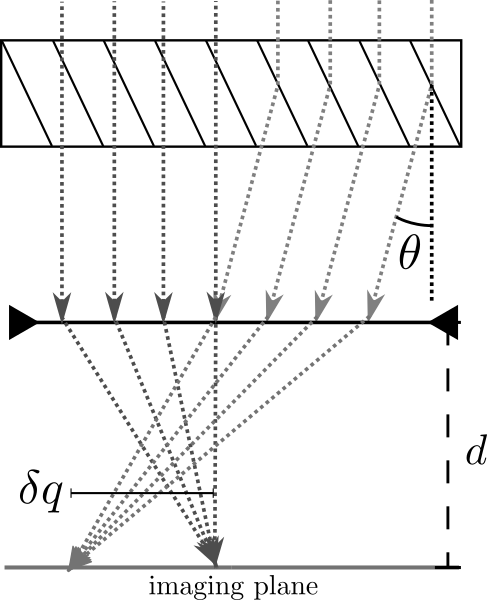
\includegraphics[width=0.8\linewidth, keepaspectratio]{Figures/diff-im.png}
	\end{minipage}%
	\begin{minipage}{0.5\linewidth}
		\centering
		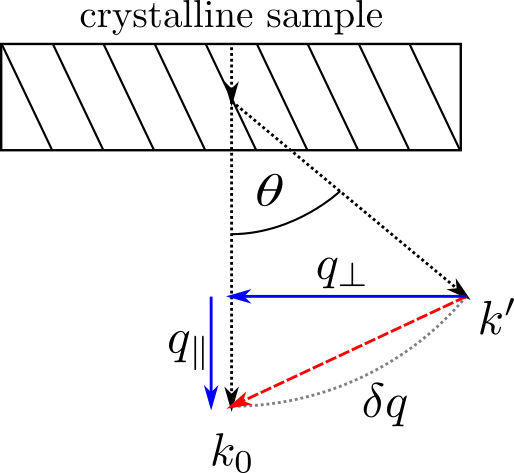
\includegraphics[width=1\linewidth, keepaspectratio]{Figures/scat.png}
	\end{minipage}
\end{frame}

\begin{frame}
	\frametitle{MR \textbf{Electron energy-loss Spectroscopy}}
	\begin{minipage}{0.5\linewidth}
		\begin{minipage}{1\linewidth}
			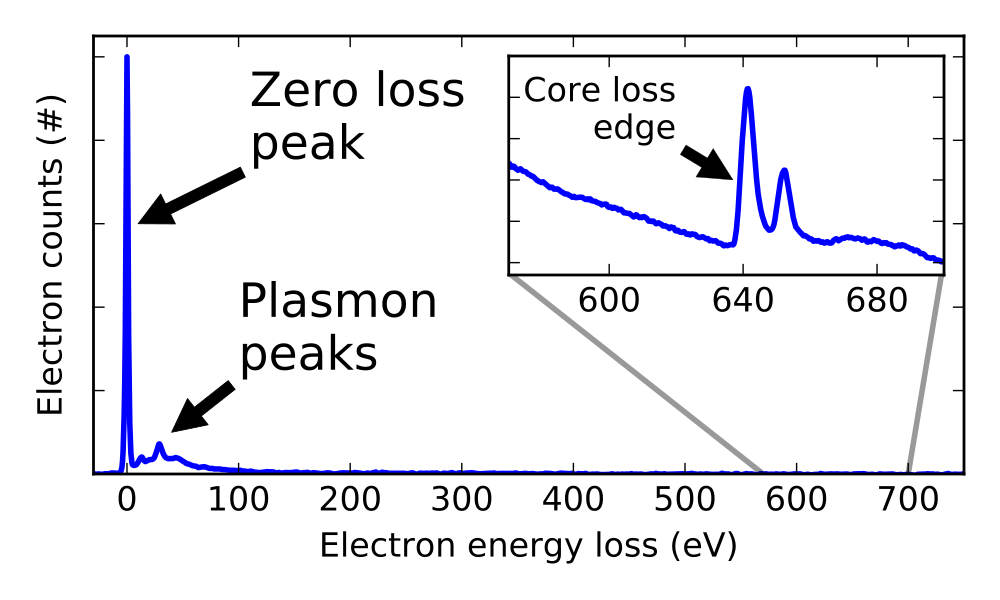
\includegraphics[width=1\linewidth, keepaspectratio]{Figures/big_eels.png}%
		\end{minipage}%
		\hfill
		\begin{minipage}{1\linewidth}
			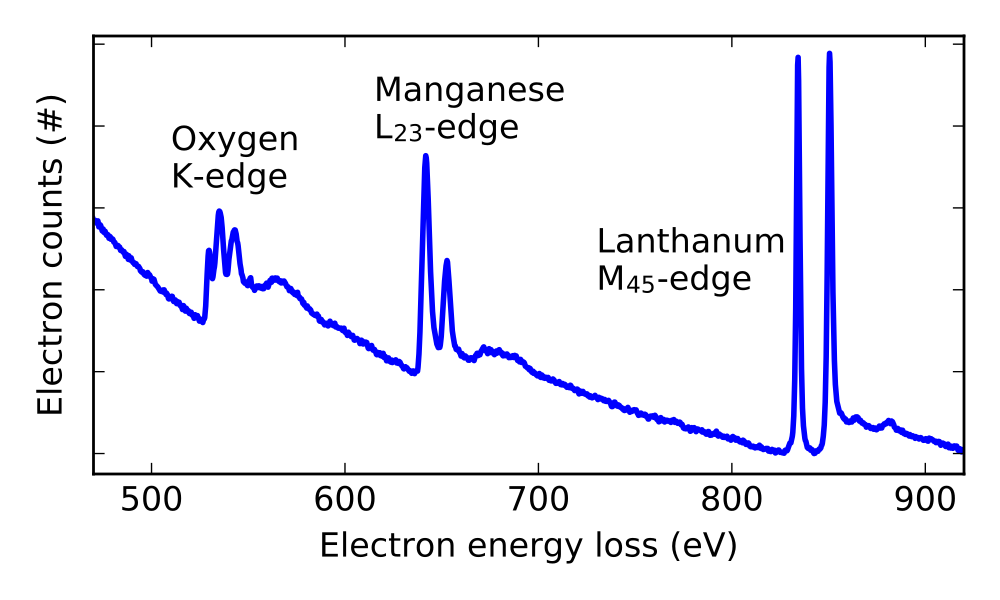
\includegraphics[width=1\linewidth, keepaspectratio]{Figures/eels-edge.png}
		\end{minipage}
		\vfill
	\end{minipage}%
	\hspace*{0.1\linewidth}
	\begin{minipage}{0.45\linewidth}
		Scattering:
		\begin{itemize}
			\item Dissimilarity in mass\\ $\rightarrow$ elastic scattering
			   \item Similar mass\\ $\rightarrow$ inelastic scattering
		\end{itemize}
		EELS use cases:
		\begin{enumerate}
			\item sample thickness measurement
   			\item electron properties
      		\item elemental analysis
		\end{enumerate}\\
	\end{minipage}
\end{frame}

\begin{frame}
	\section{Specimen}
	\frametitle{Graphene}
	\begin{minipage}{1\linewidth}
		\centering
		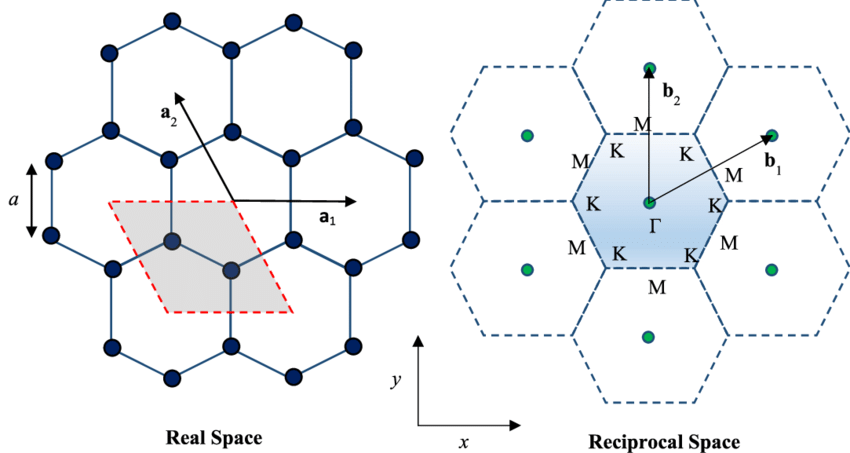
\includegraphics[width=0.9\linewidth, keepaspectratio]{Figures/graphene.png}
		\vfill
		\footnote{ \fontsize{4}{6}\selectfont Raj, Anant \& Eapen, Jacob. (2019). Phonon dispersion using the ratio of zero-time correlations among conjugate variables: Computing full phonon dispersion surface of graphene. Computer Physics Communications. 238. 10.1016/j.cpc.2018.12.008. }
	\end{minipage}
\end{frame}

\begin{frame}
	\subsection{Preparation}
	\frametitle{Sample preparation}
		Graphene easy sample
		\begin{enumerate}
			\item Mechanically exfoliated from bulk graphite
			\item Transferred onto TEM grids
			\item Baked at 500\textdegree C for 12 h in the transmission electron microscope\\ $\rightarrow$ remove contaminants
		\end{enumerate}
\end{frame}

\begin{frame}
	\subsection{Results}
	\frametitle{Setup / Results}
	\begin{minipage}{0.5\linewidth}
		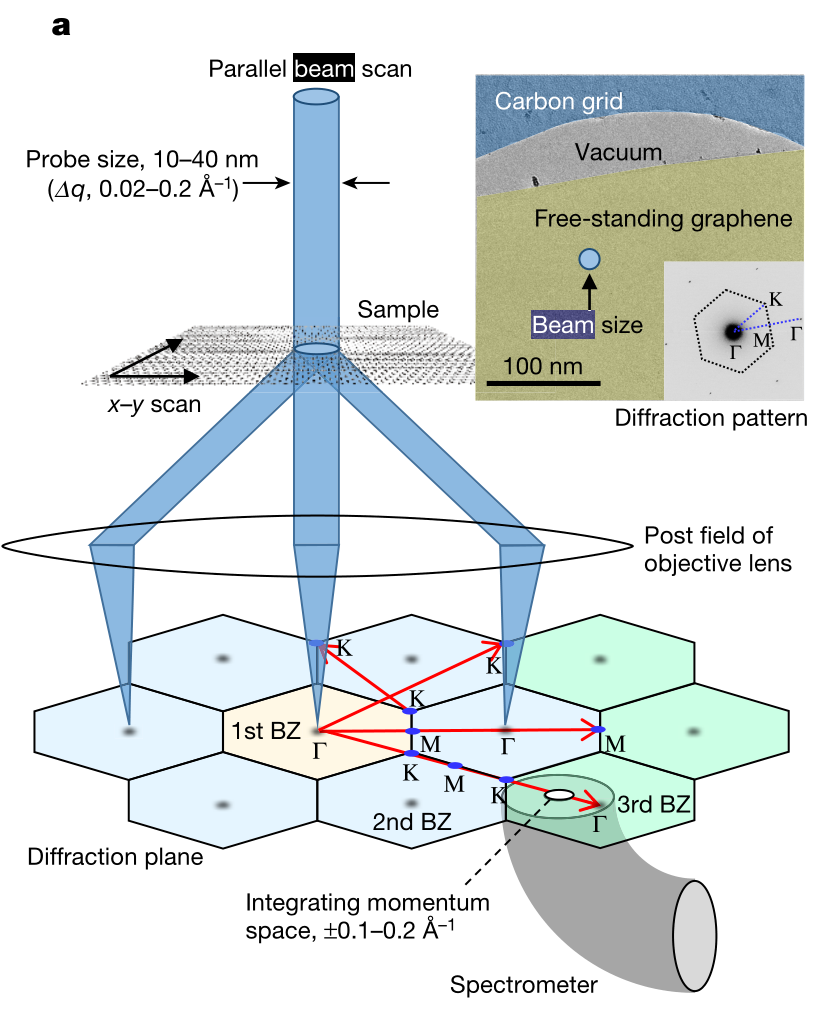
\includegraphics[width=1\linewidth, keepaspectratio]{Figures/pbs.png}
	\end{minipage}%
	\begin{minipage}{0.5\linewidth}
		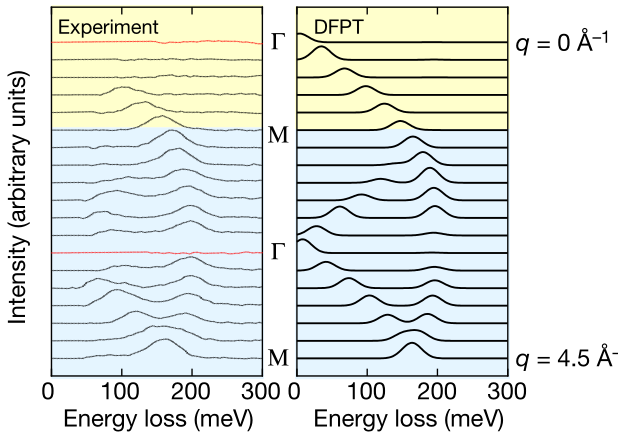
\includegraphics[width=1\linewidth, keepapsectratio]{Figures/rmap.png}
	\end{minipage}

\end{frame}

\begin{frame}
	\frametitle{Results}
	\begin{minipage}{0.7\linewidth}
		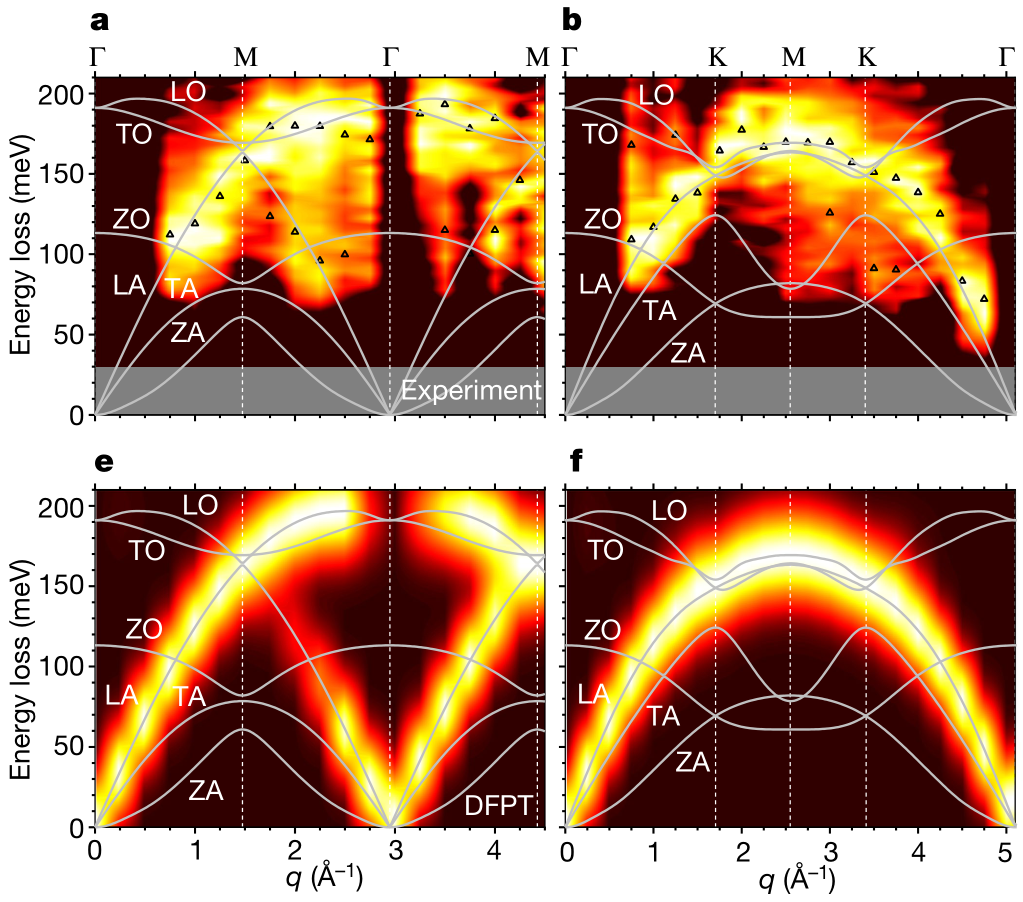
\includegraphics[width=1\linewidth, keepaspectratio]{Figures/phonon-disp.png}
	\end{minipage}%
	\begin{minipage}{0.3\linewidth}
		\begin{enumerate}
			\item many EELS spectra recorded per $q$
   			\item ordered side-by-side
   			\item peaks in spectra were tracked across $q$
		\end{enumerate}
	\end{minipage}
\end{frame}

\begin{frame}
	\section{appendix}
	\frametitle{appendix}
	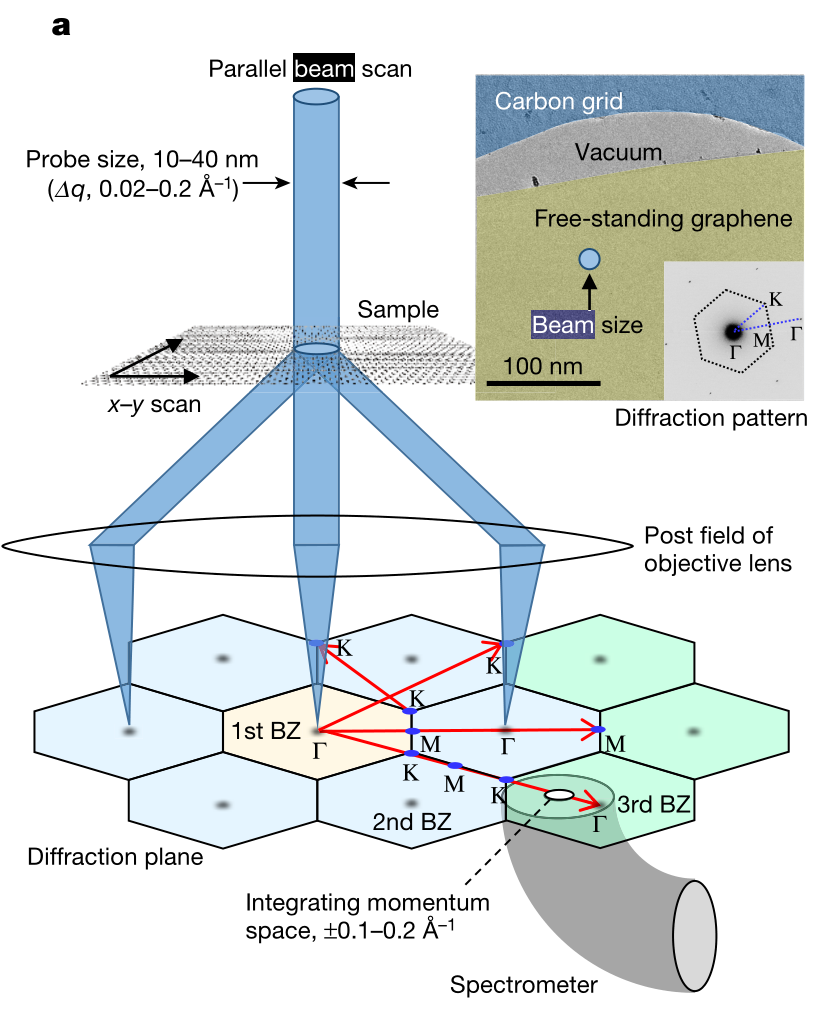
\includegraphics[width=0.6\linewidth, keepaspectratio]{Figures/pbs.png}
\end{frame}
\end{document}

